% Fichier LaTeX enrichi avec images UPDF
% Exercice 4 - Amérique du Nord ^
% 20 points

\documentclass[12pt]{article}
\usepackage[utf8]{inputenc}
\usepackage[T1]{fontenc}
\usepackage[french]{babel}
\usepackage{graphicx}
\usepackage{amsmath}
\usepackage{amssymb}
\usepackage{geometry}
\geometry{a4paper, margin=2cm}

\begin{document}

\section*{Exercice 4 (20 points)}

% Images de l'exercice
\begin{center}
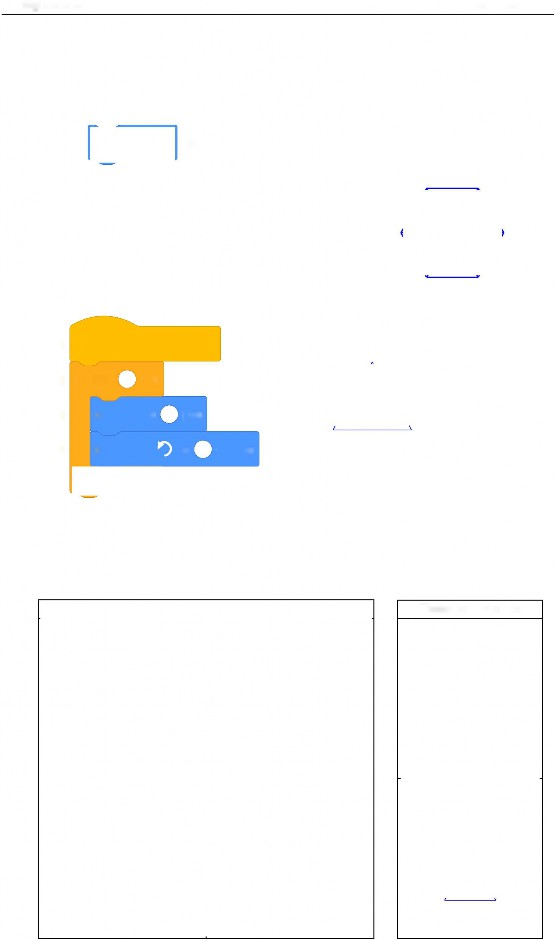
\includegraphics[width=0.8\textwidth]{images/dnb_2025_06_ameriquenord_4_Image_039.jpg}
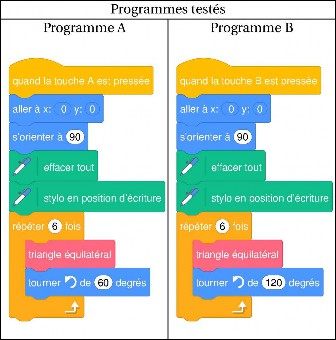
\includegraphics[width=0.8\textwidth]{images/dnb_2025_06_ameriquenord_4_Image_044.jpg}
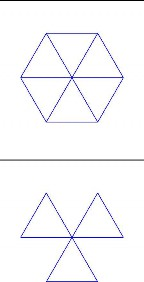
\includegraphics[width=0.8\textwidth]{images/dnb_2025_06_ameriquenord_4_Image_045.jpg}
\end{center}

\begin{enumerate}
\item Le temps et la distance parcourue par Malo sont-ils proportionnels ?

\item Quelle distance Malo a-t-il parcourue au bout de 20 minutes ?

Aucune justification n'est attendue.

\item Combien de temps a-t-il mis pour faire les 9 premiers kilomètres ?

Aucune justification n'est attendue.

\item Quelle est la vitesse moyenne de Malo lors de cette course? Exprimer le résultat au dixième de km/h près.

\item Louise et Hillal ont couru sur le même parcours de $13,5$ km. Louise à une vitesse régulière égale à $12$~km/h et Hillal a une vitesse régulière égale à $10$ km/h
\begin{enumerate}
\item[a)] Sachant que Louise et Hillal sont partis en même temps, qui a été le premier à
\item[b)] Quelle distance sépare Louise et Hillal, lorsque le premier des deux franchit la ligne d'arrivée ?
\end{enumerate}

\end{enumerate}

\end{document}
